\documentclass{article}
  % M�rgenes
  \textheight    = 20cm
  \textwidth     = 18cm
  \topmargin     = -2cm
  \oddsidemargin = -1cm
  % Sangr�a
  \parindent     =  0mm
  %Paquetes 
  %  deben venir con la distribuci�n TeX 
  %  o se pueden poner en la misma carpeta de este archivo .tex
  \usepackage{amsmath, amssymb, amsfonts, latexsym}
  \usepackage[T1]{fontenc}
  \usepackage[latin1]{inputenc}
  \usepackage{graphicx}
  \usepackage{pstricks}
  \usepackage{hyperref}
  \title{Dokumentazioa Proiektua}
  \author{Ieltzu Irazu, Mikel de Velasco, Jorge Nieto}
  \date{29 de enero de 2010}

  %Inicio del cuerpo del documento
\begin{document}
\newpage
\maketitle
\begin{center}
	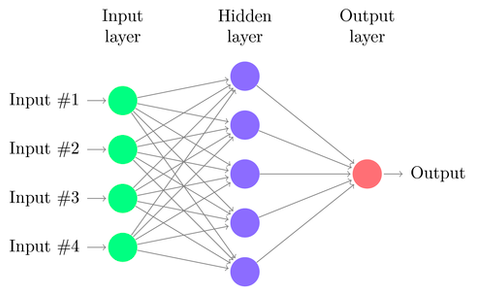
\includegraphics[width=10cm]{img/portada.png} 
\end{center}
\newpage
\section{Azaleko Orria / Aurkibidea}
\begin{enumerate}
	\item {\sc Azaleko Orria / Aurkibidea\dotfill 2}
	\item {\sc }
\end{enumerate}
\newpage
\section{Esparru Teorikoa}
\begin{enumerate}
	\item Dokumentazio eta sintesi lana landutako ikasketa teknikari buruz, alegia:
	\begin{enumerate}
	\item Support Vector Machines(SVM)
	\item {\bf Multilayer Perceptron (MP)}
	\item Bayes Network (BayesNet)
	\end{enumerate}
	Gure kasuan {\bf Multilayer Perceptron} estimatzailea ikastea tokatu zaigu. {\bf Multilayer Perceptron} ez da estimatzaile simple bat eta horregatik {\bf OneR} estimatzailearekin konparatuko dugu (estimatzaile simple dena).
	\subsection{Multilayer Perceptron}
	`Multilayer Perceptron' ingurune aldaketen aurrean aldatzen duen sare neuronal artifiziala da, eta sarrerako datu batzuetatik irteera egoki batzuetara aldatzen du. `Multilayer Perceptron' sarea hiru geruza mota desberdinetan banatzen da:
	\begin{enumerate}
		\item {\bf Sarrera geruza:} Sarean sarrera patroiak sartzen duten neurona multzoa. Neurona hauek ez dute prozesamendurik.
		\item {\bf Geruza ezkutuan:} Erdibideko neuronak dira, non bakoitzaren sarrerak aurreko geruza batetik datoz eta irteerak hurrengo geruza batera doaz.
		\item {\bf Irteera geruza:} Zeinen irteera-balioak sare guztiaren irteerekin bat datozen neuronak. 
	\end{enumerate}
	`Multilayer Perceptron' atzerako hedapen ikasketa entrenatzeko teknika erabiltzen duen sarea da. Metodo honek \href{http://en.wikipedia.org/wiki/Perceptron}{\blue{ `Estandar Linear Perceptron' }} motodoaren aldaketa bat da eta linelaki banatzeko modukoak ez diren datuak bereiz ditzake.\\\\
	{\sc \textbf{Atzerako hedapenearekin ikasten:}}\\
	Ikasketa datuak prozesatu eta gero haien pisua aldatzen denean gertatzen da, espero zen errore kopurua egon den errore kopuruarekin konparatuz.
\begin{center}
\fbox{
	\begin{minipage}[t]{15cm}
		\begin{description}
			\item[Algoritmoa:] Errorea Kalkulatu\\ (Nodo Kopurua: $N$  |  Data Puntua: $j$ | TargetValue: $d$ | Perceptroiak emandako balioa: $y$)
			\item[Aurre-baldintzak:] $n \in N$
 			\item[Emaitza:] $e_n(j)$
			\item[Begin] :\\
				$e_n(j) = d_n(j) - y_n(j)$
			\item[End]
		\end{description}
	\end{minipage}
}

\end{center}
	Errorea irteeratik sarrera joango balitz bezala ulertu daiteke, horregatik hartzen du backpropagation izena. \\\\
	{\sc \textbf{Perceptroia entrenatu:}}\\
	Perceptroiek hiperplano bat definitzen dute, eta neurona sarea perceptroiaren hiperplano hori implementatzen dute. Datu batzuk sarreratzat erabiliz, pisu balioak kalkulatu egin daitezke konexiorik gabe eta konektatzean pertzeptroiak irteera balioak kalkulatu ditu.\\
	Pertzeptroiari ez zaio lagin osoa pasatzen lehenengo aldian, honen zati bat ematen zaio. Sareak bere aldagaiak kasu bakoitzaren ostean eguneratzea da helburua, sarea gutxika definituz eta hobetuz. Errorea ez da lagin osoaren gainean kalkulatzen, baizik eta jasotako instantzia bakoitzeko errore hori txikitzen ahalegintzen da. \\
	\item Diseinua laburbildu eta atazen banaketa taldekideen artean eman. Javan garatu den programaren diseinua eta inplementazioari buruzko xehetasun aipagarrienak.
\end{enumerate}
\section{Esparru Esperimentala}
\begin{enumerate}
	\item Datuak: datuen deskribapen kualitatibo eta kuantitatiboa 2. ariketako emaitzak sartu.\\
	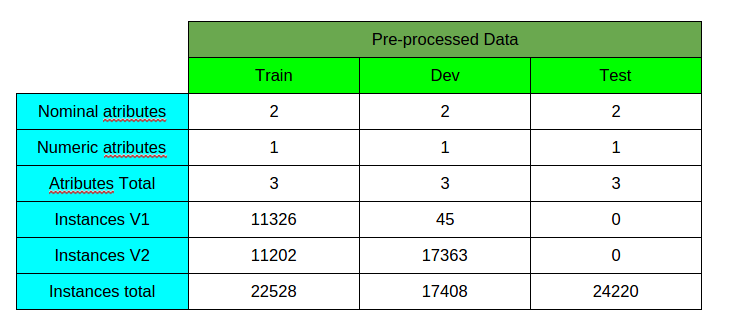
\includegraphics[width=10cm]{img/pre-process.png}
	\item Aurre-prozesamendua: erabilitako filtroak aukeratzeko motibazioa azaldu eta 3.ariketako emaitzak eman.
	\item Emaitza esperimentalak: ereduek eskaintzen duten kalitatea aztertu. ...
	\item Exekutagarrien exekuzio adibide bat (ikusi 5.1. atala).	
\end{enumerate}{
\section{Ondorioak eta etorkizunerako lana}
Lan honetan Multilayer Perceptron-ren parametro asko ekortu ditugu eta beraz oso modelo sendoa lortu dugu. Nahiz eta parametro asko ekortu izan, konturatu gara ez dela asko hobetzen modeloa. Eskatzen zeneko ia-ia guztia egin dugu eta beraz ez ditugu asko egiteko, baina etorkizuneko lan bezala beste Baseline algoritmoak ekortzea eta konparaketa berriak egitea izango zen.
\section{Bibliografia}
Bibliografia edukia indartu edo sostengatzeko emanda dago. Ezinbestekoa
da iturri bibliografikoak aipatzea erabili edo horietara jotzen garen puntuan bertan. Ez ahaztu irudien iturria aipatzen. Testuan zehar esplizituki aipatu ez den iturririk ez sartu Bibliografia atalean. Iturria aipatzean zehaztu ahalbait gehien (liburuko kapitulua edo atala eman), honela beste irakurle batek sakondu ahal izango du iturri horiek kontsultatu.
\begin{itemize}
	\item {\sc \textbf{Multilayer Perceptron:}} Data Mining - Practical Machine Learning Tools and Techniques (3rd Ed) (Page 232)
	\item {\sc \textbf{Multilayer Perceptron:}} \href{http://en.wikipedia.org/wiki/Multilayer_perceptron}{\blue{ en.wikipedia.org/wiki/Multilayer\_perceptron }}
	\item {\sc \textbf{Multilayer:}} \href{http://en.wikipedia.org/wiki/Perceptron}{\blue{ en.wikipedia.org/wiki/Perceptron }}
	
\end{itemize}

\section{Balorazio Subjektiboa}
\begin{itemize}
\item Ieltzu: Nire ustez Atazarekin lortu behar genueneko helburuak lortu dira. Denbora asko eman dut bereziki txostena egiten, gauza asko azaldu behar direlako. Ikasketarako denbora nahikotzo ere eman dut. Multilayer Perceptron nola doan jakitea denbora asko eraman dit. Diseinua egiteko ez da arazo larririk egon. Diseinua egiterakoan beharbada modeloa egiteko atala zailena izan da, luzera handienekoa da ere. Taldelana oso garrantzitzua izan da. Beti bezala, gure taldean oso ondo moldatzen gara hirurok batera eta pozik nago egindako lanarekin. Interes handiena beharbada lan handia izatearena izango da, ez genuelako hain handia den bestelako lanik egin arlo honetan.
\item Jorge:
\item Mikel:
\end{itemize}
(borondatezkoa) eranskin batean atazari buruzko hausnarketa egin. Honako puntuak lagungarriak izan daitezke baina ez dira derrigorrezkoak, beste batzuk ere sar daitezke.
\begin{enumerate}
	\item Atazarekin lortu nahi ziren helburuak lortu dituzue? (ikusi 1. atala)
	\item Batazbestean zenbat denbora eman duzue atazean lanean? Desglosatu: ikasketarako denbora, bilaketa bibliografikoa, softwarearen diseinua eta inplementazioa, txostena.
	\item Talde-lana erabilgarria izan da ataza ebazteko?
	\item Zer sortarazi dizue interesik handiena? Ikasleengan interesa eta motibazioa pizteko iradokizunak eman.   
\end{enumerate}
\newpage
\section{PROBANDO}
\begin{center}
{ \fboxsep 12pt
\fbox{
	\begin{minipage}[t]{14cm}
		\begin{description}
			\item[Algoritmoa:] NombreAlgoritmo (Entrenatzeko Instantziak: $Z$)
			\item[Aurre-baldintzak:] $Z$\hspace{1cm}$|Z| = N$
 			\item[Emaitza:] Erabaki Zuhaitza: $T$
			\item[Begin] :\\
	if( $Z$ multzoko instantzia guztiak klase berekoak dira ($C$) )\{ \\
	.\hspace{1cm}return $T$(nodo terminala (hostoa) $C$-rekin etiketatua) \\
	\} else \{ \\
	.\hspace{1cm}Haukeratu informazio gehien eskaintzen duen aldagaia $Xr (Xr = \{xr^1, ..., xr^nr\})$ \\
	.\hspace{1cm}.... \\
	.\hspace{1cm}return $T$(lotu error $Xr nr$ azpi-zuhaitzarekin: $T1, ..., Tnr$) \\
	\} \\
			\item[End]
		\end{description}
	\end{minipage}
}}
\end{center}
\end{document}
